\chapter{Задание \textnumero2}

\section{Условие}
Написать программу~--- загружаемый модуль ядра (LKM)~--- которая поддерживает чтение из пространства пользователя и запись в пространство пользователя из пространства ядра.

После загрузки модуля пользователь должен иметь возможность загружать в него строки с помощью команды echo, а затем считывать их с помощью команды cat.

В программе необходимо создать файл, поддиректорию и символическую ссылку.

\section{Реализация}

В листинге~\ref{lst:task02} приведён текст программы, реализующей данное задание.

\begin{lstlisting}[caption={Задание \textnumero2},label={lst:task02}]
#include <linux/fs.h>
#include <linux/kernel.h>
#include <linux/module.h>
#include <linux/string.h>
#include <linux/proc_fs.h>
#include <linux/vmalloc.h>
#include <linux/uaccess.h>

#define COOKIE_SIZE PAGE_SIZE

MODULE_LICENSE("GPL");
MODULE_AUTHOR("Faris Nabiev");

static int cookie_index;
static int next_fortune;
static char *cookie_pot;

static struct proc_dir_entry *p_entry;
static struct proc_dir_entry *p_dir;
static struct proc_dir_entry *p_link;

static ssize_t fortune_read(struct file *fd, char __user *buf,
                            size_t len, loff_t *ppos);
static ssize_t fortune_write(struct file *fd, const char __user *buf,
                             size_t len, loff_t *ppos);

static int fortune_init(void)
{
    static struct file_operations fops = {
        .owner = THIS_MODULE,
        .read = &fortune_read,
        .write = &fortune_write
    };

    if (!(cookie_pot = (char *)vmalloc(COOKIE_SIZE)))
    {
        printk(KERN_ERR "fortune: can't alloc memory for cookie_pot!\n");
        return -ENOMEM;
    }

    memset(cookie_pot, 0, COOKIE_SIZE);

    if (!(p_entry = proc_create("fortune", 0644, NULL, &fops)))
    {
        printk(KERN_ERR "fortune: can't create fortune entry!\n");
        vfree(cookie_pot);
        return -ENOMEM;
    }

    printk(KERN_INFO "fortune: module have loaded.\n");

    if (!(p_dir = proc_mkdir("fortune_dir", NULL)))
    {
        printk(KERN_ERR "fortune: can't create fortune directory!\n");
        return -ENOMEM;
    }
    if (!(p_link = proc_symlink("fortune_dir/fortune_link",
                                NULL, "../fortune")))
    {
        printk(KERN_ERR "fortune: can't create fortune symlink!\n");
        return -ENOMEM;
    }

    return 0;
}

static void fortune_exit(void)
{
    proc_remove(p_entry);
    proc_remove(p_dir);
    proc_remove(p_link);

    vfree(cookie_pot);

    printk(KERN_INFO "fortune: module have unloaded.\n");
}

static ssize_t fortune_read(struct file *fd, char __user *buf,
                            size_t len, loff_t *ppos)
{
    if (*ppos > 0)
        return 0;

    if (next_fortune >= cookie_index)
        next_fortune = 0;

    len = copy_to_user(buf, cookie_pot + next_fortune, len);
    next_fortune += len;
    *ppos += len;

    return len;
}

static ssize_t fortune_write(struct file *fd, const char __user *buf,
                             size_t len, loff_t *ppos)
{
    int available_size = COOKIE_SIZE - cookie_index + 1;

    if (len > (size_t)available_size)
    {
        printk(KERN_NOTICE "fortune: there is not enough "
                           "memory in cookie pot!\n");
        return -ENOSPC;
    }

    if (copy_from_user(cookie_pot + cookie_index, buf, len))
    {
        printk(KERN_NOTICE "fortune: copy_to_user failed!\n");
        return -EFAULT;
    }

    cookie_index += len;
    cookie_pot[cookie_index - 1] = 0;

    return len;
}

module_init(fortune_init);
module_exit(fortune_exit);
\end{lstlisting}

\section{Демонстрация работы}

На рисунках~\ref{img:moduleload},~\ref{img:procfiles},~\ref{img:showcase} изображены сборка, загрузка модуля, проверка созданных файлов и возможности ввода-вывода при помощи команд echo, cat.

\begin{figure}[H]
    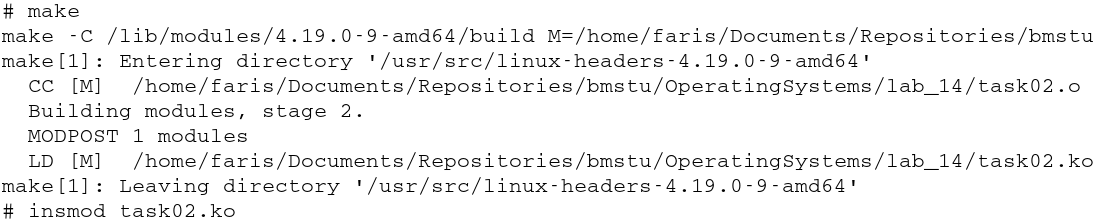
\includegraphics[scale=0.5]{images/moduleload.png}
    \caption{Сборка и загрузка модуля}\label{img:moduleload}
\end{figure}

\begin{figure}[H]
    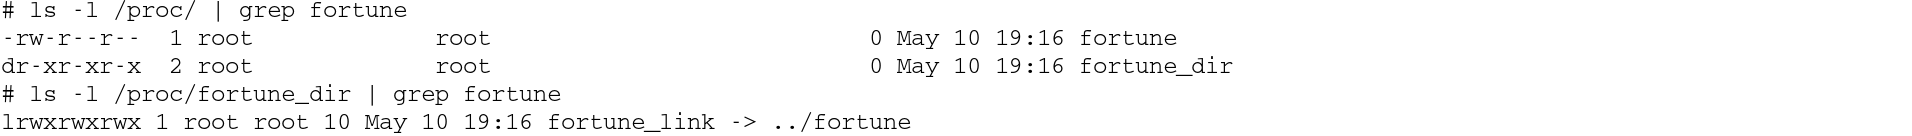
\includegraphics[scale=0.5]{images/procfiles.png}
    \caption{Проверка созданных файлов}\label{img:procfiles}
\end{figure}

\begin{figure}[H]
    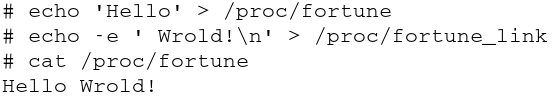
\includegraphics[scale=0.5]{images/showcase.png}
    \caption{Проверка работы}\label{img:showcase}
\end{figure}

\section{Обоснование использования\\специальных функций}
Использование copy\_to\_user, copy\_from\_user обусловлено тем, что в Linux память сегментирована. Это означает, что указатель не ссылается на уникальную позицию в памяти, а ссылается на позицию в сегменте. Процессу доступен только собственный сегмент памяти. Если выполняется обычная программа, то адресация выполняется автоматически. Если выполняется код ядра, и необходимо получить доступ к сегменту кода ядра, то всегда нужен буфер, но когда мы хотим передавать информацию между процессом и кодом ядра, то соответствующая функция ядра получит указатель на буфер процесса.

